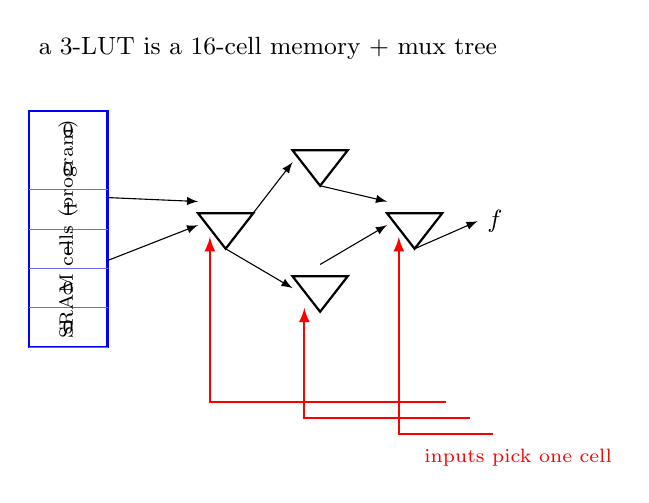
\begin{tikzpicture}[x=1cm,y=1cm, >=latex]
\node[font=\small, anchor=west] at (-0.3,3.3) {a 3-LUT is a 16-cell memory + mux tree};
% SRAM column
\draw[thick, blue] (-0.3,-0.5) rectangle (0.7,2.5);
\foreach \y in {0,0.5,...,2.49} \draw[blue!60] (-0.3,\y-0.5) -- (0.7,\y-0.5);
\node[font=\scriptsize, rotate=90] at (0.2,1.0) {SRAM cells (program)};
\foreach \y/\v in {-0.5/0,0.0/0,0.5/1,1.0/1,1.5/0,2.0/0}
  \node[font=\scriptsize] at (0.2,\y+0.25) {\v};
% mux symbols: drawn triangles (no shapes lib)
\foreach \p in {(2.2,0.75),(3.4,-0.05),(3.4,1.55),(4.6,0.75)}
  \draw[thick] \p -- ++(-0.35,0.45) -- ++(0.7,0) -- cycle;
\draw[->] (0.7,0.6) -- (1.85,1.05); \draw[->] (0.7,1.4) -- (1.85,1.35);
\draw[->] (2.2,0.75) -- (3.05,0.25); \draw[->] (2.2,0.75) -- (3.05,1.85);
\draw[->] (3.4,0.55) -- (4.25,1.05); \draw[->] (3.4,1.55) -- (4.25,1.35);
\draw[->] (4.6,0.75) -- (5.4,1.1) node[anchor=west, font=\small] {$f$};
\draw[->, red, thick] (5.0,-1.2) -| (2.0,-0.6) -- (2.0,0.9);
\draw[->, red, thick] (5.3,-1.4) -| (3.2,-0.7) -- (3.2,0.0);
\draw[->, red, thick] (5.6,-1.6) -| (4.4,-0.8) -- (4.4,0.9);
\node[red, font=\scriptsize, anchor=west] at (4.6,-1.9) {inputs pick one cell};
\end{tikzpicture}
